\documentclass[../main/main.tex]{subfiles}

\newdate{date}{23}{10}{2020}

\begin{document}

\marginpar{ \textbf{Laboratory 6.} \\  \displaydate{date}. \\ Compiled:  \today.}

Dei contatti andavano a massa quindi abbiamo dovuto smontare il campione.
Adesso facciamo il test con l'azoto. Il nostro circuito finale ha:
\begin{itemize}
\item \( R_{G} = 98.5 \, \Omega  \rightarrow G = 508.614 \);
\item \( R_0 = 4.633 \, \text{k}\Omega  \);
\item \( V_0 = 0.5 \, \text{V} \);
\item \( R_{sc}^{stimata} = 0.3 \,\Omega  \).
\end{itemize}
dove per \( R_{sc}^{stimata} \) abbiamo calcolato la resistenza del campione col multimetro semplicemente ai capi dei terminali.
Dovremmo ottenere teoricamente:
\begin{equation*}
  V_{out}^{th} = 16 \, \text{mV}
\end{equation*}
Invece otteniamo:
\begin{equation*}
  V_{out}^{mis} = 311 \, \text{mV}
\end{equation*}
C'è qualcosa che non torna. Magari la resistenza \( R_{sc} \) non è corretta, mettiamo il valore:
\begin{equation*}
  R_{sc}^{stimata} = 0.3 + 11.3 = 11.6 \,\Omega
\end{equation*}
Dovremmo ottenere teoricamente:
\begin{equation*}
  V_{out}^{th} = 600 \, \text{mV}
\end{equation*}
Questo è più in accordo con il valore misurato prima.

\begin{figure}[h!]
\centering
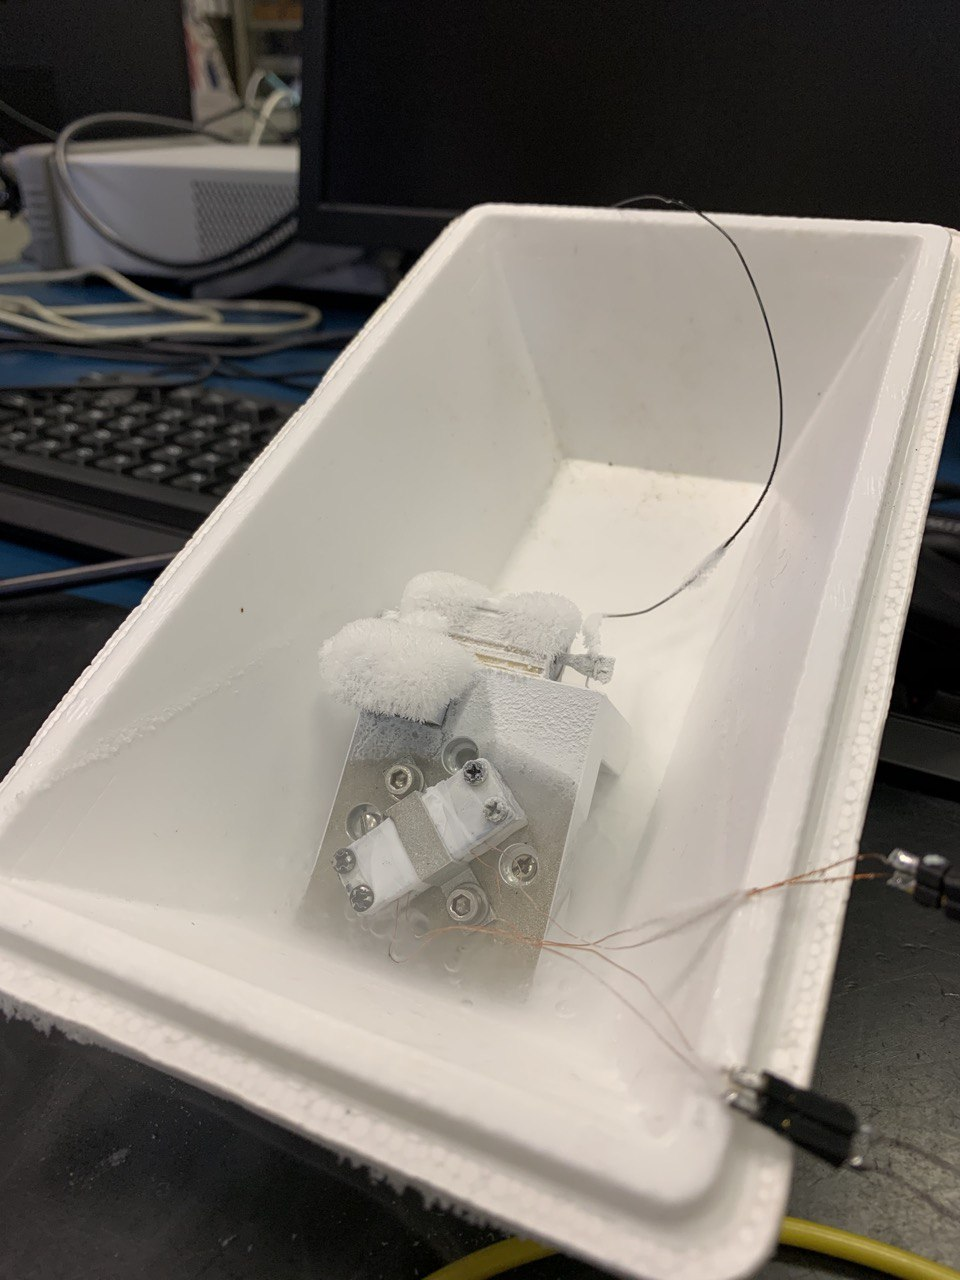
\includegraphics[width=0.6\textwidth]{../lessons/image/06/1.jpg}
\caption{\label{fig:06_1} Apparato sperimentale per il raffreddamento con l'azoto.}
\end{figure}

L'apparato sperimentale è mostrato in Fig. \ref{fig:06_1}.
L'azoto raffredda a 77 K. Versiamo l'azoto sul campione nella vaschetta di gelato. Quindi partiamo da 311 mV.
Notiamo che il voltaggio raggiunto è diventato negativo, poi è arrivato a zero, ma per poco e si è stabilizzato ai 10 mV. Poi è iniziato a risalire. E' arrivato fino a 160 mV, poi ho spostato una banana ed è sceso di nuovo improvvisamente fino a 80 mV. Abbiamo usato il phon per riscaldare. Adesso il valore è sui 180 mV. Stiamo lavorando in DC, si creano resistenze di contatto necessariemente date dal fatto che abbiamo materiali diversi, quindi non vediamo una risalita sharp ma già il fatto che il valore si stabilizzi verso 180 mV è una cosa buona. Abbiamo versato altro azoto liquido. Il voltaggio diminuisce. Non arriva perfettamente a zero il valore ma arriva a qualche mV (tipo 5 mV), questo ci sta in questo esperimento perchè possiamo avere tante resistenze parassite e altre forze elettromotrici. Secondo Mistura la presenza anche di ghiaccio crea rumori vari.
E' arrivato a a stabilizzarsi a -50 mV. L'abbiamo scaldato ed è arrivato fino a 180 mV. Abbiamo buttato altro azoto ed è transito subito perché eravamo molto vicini alla temperatura critica.
Possiamo concludere che il circuito funziona correttamente.




\marginpar{ \textbf{Laboratory 7.} \\  \displaydate{date}. \\ Compiled:  \today.}

Nell'altra lezione abbiamo ragionato sull'assemblaggio del circuito che dovrà essere saldato sul modulo NIM.




\end{document}
